\section{Marked chambers and the even cover}
\label{sec:chambers}

We now construct the data $(D,P,S,H,w)$ of
Proposition~\ref{refl:chamber-data} and verify its lifted-chamber
hypotheses and double-cover filling.  The boundary laws proved here,
together with the tensor obstruction of Section~\ref{sec:tensors},
will prove its odd-cover nonfilling assertion in
Section~\ref{sec:formal}.  The chamber construction follows
\cite[Section~2]{PD}; its new ingredient is a four-tip grope with two
red--blue pairs of tips.  We first give its marked geometric model, since
both the boundary relations and the double-cover filling depend on that
model.

\subsection{Plumbing blocks and four-tip bodies}

Fix integers
\[
 m_R=m_B=5,\qquad m=m_R+m_B,\qquad p\geq9.
\]
Start with the plumbing construction of
\cite[Section~2.2, ``The plumbing blocks'']{MT}.  Thus a four-dimensional
one-handlebody has $2m+p$ one-handles, and the first $2m$ are canceled by
two-handles with their product framings.  Before plumbing, the resulting
block $B$ is a one-handlebody on the $p$ remaining handles.  Pair the
canceling two-handles and mutually plumb each pair at a small product
patch, interchanging base and fiber.  The patches are disjoint, and
there are no self-plumbings.  Each end of a paired plumbing is called a
\emph{port}, indexed by its canceling two-handle.  Give $m_R$ plumbing
types the color red and the other $m_B$ the color blue.  Both ports
belonging to one plumbing type have the same color.

Locally the two plumbing branches are
\begin{equation}
\label{ch:plumbing-chart}
 (D^2_R\times D^2_r)\ \cup\ (D^2_r\times D^2_R)
       \subset\mathbb R^2\times\mathbb R^2,
 \qquad 0<r<R.
\end{equation}
Their overlap is the product ball $D^2_r\times D^2_r$.
The coordinate core disks $D^2_R\times\{0\}$ and
$\{0\}\times D^2_R$ meet once; separated parallel core sheets
can intersect only when they belong to opposite branches.
Rounding corners gives the smooth plumbing chart with its
product framings.

The resulting compact smooth oriented four-manifold is denoted by $X$.
Its regular cover associated to the quotient onto the plumbing group
$F_m$ consists of copies of $B$ indexed by the Cayley tree of $F_m$,
joined at product balls.  The contractible overlaps are cofibrations,
so the homotopy type is obtained by joining the block graphs along
this tree.  Passing to the quotient gives
\begin{equation}
\label{ch:plumbing-group}
 \pi_1X=F(\tau_1,\ldots,\tau_m,l_1,\ldots,l_p),
 \qquad X\simeq\bigvee^{m+p}S^1.
\end{equation}
Here $\tau_r$ crosses the join of plumbing type $r$, and the $l_s$ are
the extra handle generators.  This description also fixes the markings
in finite covers: paths through the joins are based using fixed paths
inside the blocks.

The exposed boundary piece of the block at a plumbing vertex $v$ is
\begin{equation}
\label{ch:outside-piece}
 K_v\cong\bigl(\#^p(S^1\times S^2)\bigr)
       \setminus\operatorname{int}\nu(L_{2m}),
\end{equation}
where $L_{2m}$ is an unlink in a ball.  Write
$x_i=\kappa_i m_i\kappa_i^{-1}$, where $m_i$ is the oriented meridian
at the $i$th port and $\kappa_i$ is its standard whisker from a fixed
outside basepoint.  The $x_i$ and the extra loops
$l_1,\ldots,l_p$ freely generate $\pi_1K_v$.  Each $x_i$ dies in $B$.
At a join torus the plumbing interchanges meridian and longitude, and
each longitude bounds in its own outside piece.  We suppress product
collars in this description.

Our grope body consists of a bottom punctured torus $F$, with upper
punctured tori $U_a,U_b$ attached to the respective members $a,b$ of
its symplectic basis.
The two basis curves of the first upper torus are tips $1,2$, and those
of the second are tips $3,4$.  The ordered colors of the tips are
\[
 (R,B),\quad(R,B).
\]
A cap at a tip will be a product parallel of the core belonging to its
assigned port.  Figure~\ref{ch:grope-figure} records the incidence and
color data; it does not depict an embedding.

\begin{figure}[ht]
\centering
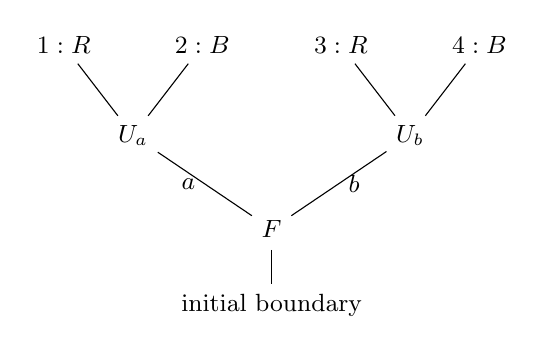
\begin{tikzpicture}[scale=.88,every node/.style={font=\small}]
 \node (F) at (0,0) {$F$};
 \node (A) at (-2,1.35) {$U_a$};
 \node (B) at (2,1.35) {$U_b$};
 \node (r1) at (-3,2.65) {$1:R$};
 \node (b2) at (-1,2.65) {$2:B$};
 \node (r3) at (1,2.65) {$3:R$};
 \node (b4) at (3,2.65) {$4:B$};
 \draw (F)--node[left]{$a$}(A);
 \draw (F)--node[right]{$b$}(B);
 \draw (A)--(r1) (A)--(b2) (B)--(r3) (B)--(b4);
 \draw (0,-.3)--(0,-.8);
 \node at (0,-1.1) {initial boundary};
\end{tikzpicture}
\caption{The four-tip body.  At a vertex where red ports are selected,
each upper torus can be compressed using its red cap; at the other
vertex of the double cover, both compressions use blue caps.}
\label{ch:grope-figure}
\end{figure}

Put $\mathcal C=\{1,l_1,\ldots,l_p\}$.  Install one body for every
ordered quadruple $(i_1,i_2,i_3,i_4)$ of distinct ports with colors
$(R,B,R,B)$, every independent choice $c_\alpha\in\mathcal C$, and
every independent sign $\varepsilon_\alpha\in\{1,-1\}$.  Its based
tips must represent
\begin{equation}
\label{ch:tip-markings}
 X_\alpha=c_\alpha x_{i_\alpha}^{\varepsilon_\alpha}c_\alpha^{-1},
 \qquad 1\leq\alpha\leq4,
\end{equation}
in the outside piece.  There are finitely many bodies; denote their
number by $k$, and use the same list in every translate of a block.

\begin{lemma}[The four-tip marked body]
\label{ch:four-tip-model}
The four-tip body has a three-dimensional handlebody thickening that,
with its four marked tip annuli, is a boundary connected sum of four
solid tori with longitudinal marked annuli.  The finite list above can
be placed with disjoint bodies and the markings
\eqref{ch:tip-markings} in the outside pieces of the plumbing.
The bottom surfaces are proper inward pushes of disjoint boundary
surfaces of $X$.  Each terminal cap is embedded and framed; it misses
all body sheets away from its own attachment.  The only possible
cap--cap intersections occur between opposite ports of a plumbing.
\end{lemma}

\begin{proof}
We extend the marked three-tip model of
\cite[Lemma~2.3]{MT}.  Thicken a punctured torus to its product with
an interval and put its two basis annuli on opposite faces.  Two
disjoint cutting arcs, each dual to one basis curve and disjoint from
the other, give disjoint meridian disks in the product.  To see these
arcs explicitly, puncture the square torus near $(1/2,1/2)$, take
the basis circles at $x=1/4$ and $y=1/4$, and cut along the arcs
at $y=1/2$ and $x=1/2$.  The puncture removes their only mutual
intersection.  Each product disk meets its own marked annulus in
one essential arc and misses the other.

Cutting the thickening along these disks gives a ball.  Each marked
annulus becomes a rectangle joining the two faces of its own cutting
disk.  The rectangle and those two disk faces have a disk neighbourhood
in the boundary sphere, disjoint from the analogous neighbourhood for
the other annulus.  A boundary homeomorphism, extended over the ball,
identifies this marked configuration with the standard one.  After
reattaching the handles, the lower thickening is therefore a boundary
connected sum of two longitudinal-annulus collars.  This is a statement
about the annuli themselves, not just their elements of the free group.

Attach an upper punctured-torus thickening along each of these two
annuli.  A longitudinal-annulus collar is a solid torus viewed as an
annulus times an interval; gluing it on merely collars the attaching
annulus of its upper thickening.  The single boundary-sum tube of the
lower model now joins the two upper thickenings.  Extend the two
meridian disks from each upper thickening through its own collar.
The feet of the joining tube can be chosen arbitrarily small in the
complement of the attaching annuli and moved away from the finitely
many extending disk strips.  The four extended disks are thus disjoint
and dual to the four tip annuli.  Cutting along them and repeating the
preceding ball argument proves the asserted four-tip marked model.
There is only one joining tube between the upper handlebodies, so no
additional free generator is introduced.  The initial boundary and
all the surface markings are transported with this identification.

For placement we use the refinement of
\cite[Section~2.2, ``The exterior with its side marking'']{PD}:
place the bodies in the complement of sufficiently thin attaching
solid tori in the initial one-handlebody boundary, and lengthen only
the returning tip collars to the attaching regions.  The connectors
and their basing paths then lie in $K_v$ after plumbing.  Reserve
separated product parallels of the attaching curves, one for each
occurrence of a tip, and join their thin longitudinal collars by
tubes along a rooted tree.  Let $\eta$ run from the outside basepoint
to its root and let $p_\alpha$ be the tree path from that root to
the $\alpha$th tip collar.  Choose these paths so that
$\eta p_\alpha$ is homotopic relative to its endpoints to
$c_\alpha\kappa_{i_\alpha}$, using the product tracks to identify
the parallel meridians.  Then
\[
 (\eta p_\alpha)m_{i_\alpha}^{\varepsilon_\alpha}
       (\eta p_\alpha)^{-1}
   =c_\alpha x_{i_\alpha}^{\varepsilon_\alpha}c_\alpha^{-1}
   \quad\text{in }\pi_1K_v.
\]
There is no compatibility restriction among the four chosen classes:
finitely many arcs in a three-manifold can realize them disjointly
away from their common root, with parallel tracks for repeated
portions and with the reserved returning strips avoided.  The tree
paths fix the required basing; other paths inside the resulting
handlebody add only words in its four tip generators.  The initial
boundaries remain in the outside pieces, and the bottom surfaces
are proper pushes of disjoint boundary surfaces of $X$.

We finally specify the framings.  The surface-product model frames a
surface by its oriented normal in the three-dimensional body and the
collar direction.  At a terminal annulus use the framing adjustment
in the proof of \cite[Lemma~2.3]{MT}, before fixing the returning
collar.  In a separated solid-torus neighbourhood this is the ribbon
twist
\[
 (\theta,z)\longmapsto(\theta,e^{in\theta}z).
\]
Replace $e^{in\theta}$, if necessary, by a smooth degree-$n$ circle map
$\phi(\theta)$ equal to $1$ near the connector feet.  The twist is
then the identity at those feet and extends by the identity over
the joining tubes.  Apply it to the complete marked body, including
the initial boundary and the lower and upper attaching annuli.

The returning collar is constructed after this transport.  In
coordinates $S^1_\theta\times D^2_z\times[0,1]_u$, choose an embedded
smooth regular plane arc $(r(s),u(s))$ from $(0,0)$ to $(0,1)$, departing in the
positive $r$ direction and vertical near its endpoint, with $u$
strictly increasing for $s>0$.  The collar
\[
 (\theta,s)\longmapsto
       (\theta,r(s)i\phi(\theta),u(s))
\]
leaves the transported surface ribbon in its outgoing normal
direction and ends at the same product circle $z=0,u=1$.  Its
normal quotient has frame
\[
 v=\phi(\theta),\qquad
 w=r'(s)\partial_u-u'(s)i\phi(\theta).
\]
At the first end this is the surface-transverse and collar frame;
at the last, up to a fixed constant change of frame, it has winding
$n$ relative to the core product frame.
Choose $n$ to match those framings.  The four disjoint longitudinal
neighbourhoods make the adjustments independent and leave the
external basing paths fixed.  The initial-boundary link and its
surface framing are fixed after these transports.  At each of the
three symplectic pairs, the attachments depart on opposite normal
sides.  Put the bodies at an inner collar level and extend the tips
into separated product parallels of the handle cores.  The collar
separation and the plumbing charts give the final assertions.
\end{proof}

We use the group commutator convention $[x,y]=xyx^{-1}y^{-1}$.

\begin{lemma}[The boundary laws]
\label{ch:laws}
For each installed body, its initial boundary represents, up to overall
conjugation, a word $L$ in the four based tips satisfying
\begin{equation}
\label{ch:law-properties}
 L\big|_{X_\alpha=1}=1\quad(1\leq\alpha\leq4),
 \qquad
 L\equiv [[X_1,X_2],[X_3,X_4]]
       \pmod{\Gamma_5 F(X_1,X_2,X_3,X_4)}.
\end{equation}
Here $\Gamma_r$ is the lower central series, and orientations are
chosen for the displayed sign.
\end{lemma}

\begin{proof}
The boundary of a punctured torus is the commutator of its based
symplectic generators.  Apply this first to the two upper tori and
then to the bottom torus.  Internal paths may conjugate a tip or an
upper commutator by words in the four tips.  Such conjugations change
the weight-four expression only in weight at least five.  If any
one tip is set equal to the identity, the commutator at its upper
torus becomes trivial, and then so does the bottom commutator.
These are word identities in the abstract tips; substituting the
markings \eqref{ch:tip-markings} gives the corresponding
initial-boundary words in $\pi_1K_v$.
\end{proof}

\subsection{The exterior and its homotopy type}

Write $F_1,\ldots,F_k$ for the bottom punctured tori, and $a_j,b_j$
for their two branch curves.  Both branch curves are null-homotopic
in $X$: an upper punctured torus and its terminal caps give a
null-homotopy.  Since $F_j$ retracts to its two branch curves and
$X$ has graph homotopy type, the entire map $F_j\to X$ is
null-homotopic.

Remove the interiors of disjoint product tubes of the $F_j$, including
their proper boundary collars, and put
\[
 E=X\setminus\bigcup_{j=1}^k\operatorname{int}\nu(F_j).
\]
The tubes can be chosen to avoid the upper caps and meet the upper
surfaces only along short attaching collars.  The exterior is
connected, since paths can be moved off the proper codimension-two
surfaces and then off sufficiently thin tubes.

The surface-product trivializations specify the following input from
\cite[Lemma~2.2]{PD}.

\begin{lemma}[The marked exterior model]
\label{ch:exterior-model}
There is a homotopy-pushout model
\begin{equation}
\label{ch:exterior-pushout}
 E\simeq X\cup_{\coprod_jF_j}\coprod_j(F_j\times S^1),
\end{equation}
where $F_j$ maps to $F_j\times S^1$ by its inward section.  Under
this model the displayed maps from $F_j\times S^1$ are the actual
tube-side maps, and $S^1$ is the normal circle.
\end{lemma}

The marking of the side maps is essential here.  The hypotheses of
the cited lemma hold because Lemma~\ref{ch:four-tip-model} places
the $F_j$ as proper pushes of disjoint boundary surfaces with their
surface-product trivializations.  The model can be seen in a boundary
collar: the outer part of the exterior contributes a bridge across
the deleted surface, while its inward normal semicircle supplies a
specified return path in the inner $X$ piece.  The bridge followed
by that return is exactly the tube's normal circle.  This identifies
the section and side maps in \eqref{ch:exterior-pushout}, as required
for the following gluing.

For each $j$, regard a solid torus $V_j$ as a compression body from
$F_j$ to a disk, compressing $a_j$.  Define
\begin{equation}
\label{ch:chamber-definition}
 D=E\cup_{\coprod_j(F_j\times S^1)}
             \coprod_j(V_j\times S^1),\qquad S=\partial D,
\end{equation}
using the product framings and rounding corners.  The remaining disk
face of $V_j$ contributes a solid torus to $S$.  Hence $S$ is the
surface-framed surgery of $\partial X$ along the initial-boundary
link.  In particular, $S$ is connected.

\begin{proposition}[The chamber homotopy type]
\label{ch:homotopy-type}
With the markings induced by the preceding construction,
\begin{equation}
\label{ch:group-and-spheres}
 H:=\pi_1D=\pi_1X*F(z_1,\ldots,z_k),\qquad
 D\simeq BH\vee\bigvee^{2k}S^2,
\end{equation}
where $BH$ is a finite graph and $z_j$ is the normal-circle generator
of the $j$th replacement.  On the common surgery-link exterior in
the boundary, killing the $z_j$ recovers the original marking into
$\pi_1X$.
\end{proposition}

\begin{proof}
The side-marked model of Lemma~\ref{ch:exterior-model} gives
\[
 D\simeq X\cup_{\coprod_jF_j}\coprod_j(V_j\times S^1).
\]
Because each attaching map $F_j\to X$ is null-homotopic, the
additional based summand is the homotopy cofiber of
$F_j\to V_j\times S^1$.  Retract $V_j\times S^1$ to the torus
on its longitude $b_j$ and normal circle $z_j$.  Since $F_j$
retracts to $a_j\vee b_j$, its cone adds one two-cell on the
trivial loop $a_j$ and another killing $b_j$.  Cancel the latter
one/two-cell pair.  The old torus two-cell, originally attached
by $[b_j,z_j]$, now has trivial attaching map.  The cofiber is
therefore
\[
 S^1_{z_j}\vee S^2\vee S^2.
\]
This proves \eqref{ch:group-and-spheres}.  The model retains the
normal-circle marking, so its quotient killing the new generators
is the old $X$-marking.  Equivalently, the classifying map to the
graph of $X$ extends over each replacement, since both $a_j$ and
$b_j$ map trivially and the new normal circle is sent to the
identity.  Its restriction to the common boundary exterior is the
original classifying map.
\end{proof}

\subsection{The middle form and the Poincar\'e chamber}

We next identify the entire middle homotopy module by framed
hyperbolic pairs.  This serves two purposes: it produces the
graph-type Poincar\'e pair required for reflection, and it makes
the double-cover filling an explicit geometric operation.
All intersection pairings below use fixed whiskers and the
involution $h\mapsto h^{-1}$ on the group ring.

Compress either upper punctured torus along either one of its
terminal caps.  Cutting the torus along that basis curve gives a
pair of pants, whose two new boundary curves are filled by opposite
parallel copies of the selected cap.  The result is an embedded
framed disk along the corresponding bottom branch, subject only
to intersections with other selected cap sheets.  The unused cap
does not belong to this disk.  The outgoing collar and its framing
are the local compression model of \cite[Lemma~2.4]{MT}.  At the
bottom torus the two upper attachments use distinct normal angles,
so this construction applies simultaneously on the $a_j$- and
$b_j$-branches.

\begin{lemma}[Algebraic duals]
\label{ch:exterior-duals}
There are proper framed immersed disks $f_j$ in $E$, bounded by
the truncated $a_j$-branch curves, and framed spheres $g_j$ in $E$
such that
\begin{equation}
\label{ch:dual-pairings}
 \lambda(f_i,g_j)=\delta_{ij},\qquad
 \lambda(g_i,g_j)=0
 \quad\text{over }\mathbb Z[\pi_1E].
\end{equation}
Each $g_j$ is embedded with trivial normal bundle.  If all terminal
caps selected for the branch compressions are mutually disjoint,
these representatives have exactly one geometric intersection
between $f_j$ and $g_j$ and no other intersections.
\end{lemma}

\begin{proof}
Choose one terminal cap on each upper torus.  Let $f_j$ be the
proper truncation of the compression disk on the $a_j$-branch, and
let $C_j$ be the compression disk on the $b_j$-branch.  Near the
tube side over $b_j$, take the normal-circle torus and compress it
with two parallels of $C_j$.  Denote the resulting sphere by $g_j$.

Here is the local collar calculation, from
\cite[Lemma~2.4]{MT}, that also checks its applicability to the
new $a_j$-branch.  Use coordinates $(s,t,r,\theta)$, where $s$
runs along $b_j$, $t$ is transverse to $b_j$ in $F_j$, and
$(r,\theta)$ are polar coordinates normal to $F_j$.  The rim
torus is $t=0$, $r=\rho$.  The outgoing $a_j$-disk collar and
the $b_j$-upper attachment have distinct angles
$\theta_A,\theta_B$.  Cut the rim torus at a narrow band around
$\theta_B$ and keep the annulus containing $\theta_A$.  Place
the interiors of its two compression disks outside $r=\rho$.
The retained annulus meets the $a_j$-disk collar once.  Orient
and base this point to contribute $1$.  This calculation only
uses the outgoing framed collar of that disk, so it remains
valid when the disk itself is obtained by upper-torus compression.
The disjoint body neighbourhoods exclude collar intersections
between different indices.

Every remaining intersection occurs in a cap--cap plumbing chart.
Within $g_j$, label the two copies of $C_j$ by
$\epsilon\in\{+1,-1\}$ and the two cap sheets in a fixed copy
by $\eta\in\{+1,-1\}$.  Their orientation coefficients are
$\epsilon\eta$.  Fix $\epsilon$ and an opposing sheet.  The
whisker on the opposing sheet is held fixed in this comparison.
The two paths on $g_j$ share the whole stem from the rim to the
fixed copy of $C_j$ and split only inside its upper torus.  Their
difference there is the other basis loop, which bounds the
unused terminal cap in $E$: no upper cap was removed with the
bottom tubes.  A small normal turn around the upper surface
also bounds in $E$, because that surface has not been deleted.
The two intersection labels are consequently the same element
$h\in\pi_1E$, and their contributions cancel as
\[
 \epsilon\eta h+\epsilon(-\eta)h=0.
\]
Figure~\ref{ch:sheet-cancellation} displays the two cancellations.
The outer index $\epsilon$ is fixed throughout this cancellation;
we make no identification of paths that differ by a bottom
normal circle.  The opposing sheet may come either from another
rim sphere or from the compressed $a$-branch.  This proves
\eqref{ch:dual-pairings}.

\begin{figure}[ht]
\centering
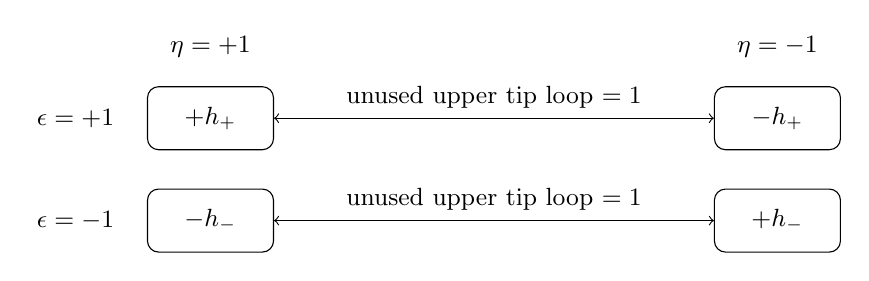
\begin{tikzpicture}[x=1cm,y=1cm,every node/.style={font=\small},
 contribution/.style={draw,rounded corners,minimum width=16mm,minimum height=8mm}]
 \node at (0,2.2) {$\eta=+1$};
 \node at (7.2,2.2) {$\eta=-1$};
 \node[anchor=east] at (-1.1,1.3) {$\epsilon=+1$};
 \node[anchor=east] at (-1.1,0) {$\epsilon=-1$};
 \node[contribution] (pp) at (0,1.3) {$+h_+$};
 \node[contribution] (pm) at (7.2,1.3) {$-h_+$};
 \node[contribution] (mp) at (0,0) {$-h_-$};
 \node[contribution] (mm) at (7.2,0) {$+h_-$};
 \draw[<->] (pp)--node[above]{unused upper tip loop $=1$}(pm);
 \draw[<->] (mp)--node[above]{unused upper tip loop $=1$}(mm);
\end{tikzpicture}
\caption{The four cap-sheet contributions in $g_j$, for one fixed
opposing sheet and up to its common intersection sign.  Rows index
the outer parallel copies of $C_j$ by $\epsilon$; columns index the
inner cap parallels by $\eta$.  The unused cap identifies the two
group labels within each row, so that row cancels.  No comparison
between $h_+$ and $h_-$ is made: the paths for different rows can
differ by a bottom normal circle.  This is a diagram of contributions,
not a projection of embedded surfaces, following the sheet calculation
in \cite[Lemma~2.4]{MT}.}
\label{ch:sheet-cancellation}
\end{figure}

A rim sphere uses only parallel copies of a single selected
terminal cap.  That core has no self-plumbing.  The separated
collars therefore make each sphere embedded, and the product
compression framings give its trivial normal bundle.  If the
selected caps are all disjoint, there are no plumbing
intersections at all; the single collar intersection in each
pair is then the complete geometric intersection set.
\end{proof}

Close $f_j$ by the meridian disk of $V_j$ at its fixed normal-circle
coordinate, obtaining a sphere $u_j\subset D$.  The framings agree:
on the $f_j$ side the frame is transverse to $a_j$ inside $F_j$
together with the circle direction, while on the meridian-disk
side it extends as the solid-torus transverse direction and the
product-circle direction.  Thus $u_j$ is framed.  Lemma~\ref{ch:exterior-duals}
gives
\begin{equation}
\label{ch:middle-pairings}
 \lambda(u_i,g_j)=\delta_{ij},\qquad
 \lambda(g_i,g_j)=0
 \quad\text{over }\Lambda:=\mathbb ZH.
\end{equation}

\begin{proposition}[The Poincar\'e chamber]
\label{ch:poincare-chamber}
The manifold $D$ has a specified framed immersed hyperbolic basis
for its full module $\pi_2D$, with vanishing quadratic
self-intersections.  Attach one three-cell on each of these
$2k$ basis spheres, and call the resulting space $P$.  Then
$(P,S)$ is an oriented finite four-dimensional Poincar\'e pair,
the inclusion $(D,S)\to(P,S)$ preserves the fundamental group
and the boundary, and $P\simeq BH$.
\end{proposition}

\begin{proof}
We give the middle-form verification used in
\cite[Section~2.3, ``The middle form and the Poincar\'e pair'']{PD}.
The hermitian matrix of the $u_i$ has even identity coefficient
on its diagonal, since their normal framings give zero
Stiefel--Whitney evaluations.  The free group $H$ has no
nonidentity element of order two.  Hence each diagonal entry
can be written $z+\overline z$: choose one coefficient from
each nonidentity inverse pair and halve the even identity
coefficient.  Subtracting suitable $\Lambda$-linear combinations
of the $g_j$ from the $u_i$, using a triangular half off the
diagonal and these halves on the diagonal, makes all pairings
among the modified $u_i$ vanish.  The cross-pairings and the
$g_i,g_j$ pairings in \eqref{ch:middle-pairings} are unchanged.

Represent these classes by immersed spheres using the usual
tubing operations.  Their even normal parity permits framed
representatives.  Write $\mu$ for the full framed Wall invariant
in the additive quotient
\[
 \Lambda/\langle h-h^{-1}:h\in H\rangle_{\mathbb Z};
\]
in particular, its identity coefficient is retained.  For a framed
representative, the symmetrization identity
\[
 \lambda(v,v)=\mu(v)+\overline{\mu(v)}
\]
and the absence of order-two elements show that its Wall
quadratic self-intersection is zero when its self-pairing
vanishes.  This is the framed immersed-sphere calculation in
the cited section; no embedded-surgery theorem is used.
Write $A_j,B_j$ for the resulting hyperbolic pairs.

They form a basis of the whole module.  By
Proposition~\ref{ch:homotopy-type}, $\pi_2D$ is free of rank
$2k$ over $\Lambda$.  Relative to any such basis, the square
matrix with columns $A_j,B_j$ has a left inverse supplied by
its nonsingular hyperbolic pairing.  Matrix rings over
$\mathbb ZH$ are directly finite: pass a one-sided inverse
identity to every finite quotient of $H$, use the finite
dimensional regular representation over $\mathbb C$ to obtain
the reverse identity, and then use residual finiteness to
separate the finite support of any nonzero group-ring entry.
The matrix therefore has a two-sided inverse.

A map from $BH\vee\bigvee^{2k}S^2$ to $D$ realizing this
basis is a homotopy equivalence: it induces the marked
isomorphism on $\pi_1$ and an isomorphism on the homology of
the simply connected covers.  Attaching the indicated
three-cells cancels the sphere summands in that homotopy
type.  Thus $P\simeq BH$.

For completeness, the duality argument of \cite[Section~2.3]{PD}
applies to exactly this basis.  The middle sphere module of
$D$ maps isomorphically to a split summand of
$H_2(D,S;\Lambda)$ by its nonsingular intersection form.
The three-cell attachments quotient the absolute and relative
middle homology by these summands; their attaching map is
injective on the summands, so no new third homology appears.
In cohomology the pullbacks identify the new groups with the
annihilators of the sphere summands.  If $i:(D,S)\to(P,S)$ is
the inclusion and $[P,S]=i_*[D,S]$, cap-product naturality
gives
\[
 \alpha\frown[P,S]
   =i_*\bigl(i^*\alpha\frown[D,S]\bigr).
\]
The duality isomorphisms for $(D,S)$ consequently induce
duality on these annihilators and quotients.  The finite
free chain complexes over $\Lambda$ give the regular-coefficient
criterion for Poincar\'e duality with all local coefficients.
This proves the assertion for $(P,S)$, with its original
boundary collar and orientation.
\end{proof}

\begin{corollary}[Connected lifted boundary]
\label{ch:boundary-surjectivity}
The boundary marking $\pi_1S\to H$ is surjective.
\end{corollary}

\begin{proof}
Duality for $(P,S)$ and the graph homotopy type of $P$ give
\[
 H_1(P,S;\mathbb ZH)=H_0(P,S;\mathbb ZH)=0.
\]
Therefore
$H_0(S;\mathbb ZH)\to H_0(P;\mathbb ZH)$ is an isomorphism.
The source is free abelian on the cosets of the image of
$\pi_1S$, whereas the target is $\mathbb Z$.  There is only
one coset.
\end{proof}

\subsection{Cyclic covers and marked fillings}
\label{ch:cyclic-covers}

Define the epimorphism
\begin{equation}
\label{ch:cover-character}
 w:H\longrightarrow\mathbb Z,\qquad
 w(\tau_r)=1,\quad w(l_s)=w(z_j)=0.
\end{equation}
For $d\geq1$, let
\[
 H_d=\ker(H\xrightarrow{w}\mathbb Z\longrightarrow\mathbb Z/d),
\]
and denote the associated connected covers by $D_d,P_d,S_d$.
We also write $X_d$ for the plumbing cover obtained by restricting
$w$ to $\pi_1X$.  The plumbing graph of $X_d$ has vertices
$\mathbb Z/d$, an edge of each type $r$ from $v$ to $v+1$,
and $p$ extra loops at every vertex.  Its bodies are copies of
the full marked list at each vertex.

\begin{lemma}[Persistence of the chamber data]
\label{ch:cover-data}
For every $d$, the data $(D_d,P_d,S_d,H_d)$ satisfy
Propositions~\ref{ch:homotopy-type} and~\ref{ch:poincare-chamber}
with all the bodies and basis spheres lifted.  In particular,
$S_d$ is connected, $H_d$ is free, $P_d\simeq BH_d$, and
$(P_d,S_d)$ is the oriented Poincar\'e pair obtained by
attaching three-cells to a specified framed immersed
hyperbolic basis of $D_d$.
\end{lemma}

\begin{proof}
Corollary~\ref{ch:boundary-surjectivity} gives connectedness
of $S_d$.  The side-marked exterior model identifies the
covering character on $\pi_1E$ with the one inherited from
$X$, with each normal circle sent to zero.  Its restriction
to $\pi_1(V_j\times S^1)$ is trivial: the longitude maps
trivially in $H$ and $w(z_j)=0$.  Thus the cover of each
replacement is trivial, and performing the chamber
construction on every lifted body in $X_d$ gives $D_d$.
The cofiber calculation is unchanged.

Each basis sphere has $d$ lifts.  Algebraically, the universal
cover is the same and its free middle module is restricted
from $\mathbb ZH$ to $\mathbb ZH_d$.  Pairings of two
chosen lifts are obtained by taking, in the pairing of their
corresponding coset translates, the coefficients supported
in $H_d$.  The lifted hyperbolic pairings are therefore standard.
The Wall invariant of a chosen lift is obtained, after the corresponding
change of whisker, by retaining precisely the self-intersection labels
in $H_d$.  Because $H_d$ is closed under inversion, this additive
coefficient projection retains the identity and both members of every
retained inverse pair.  It therefore descends to the framed Wall
quotient and carries the zero downstairs invariant to zero.
The lifted sphere classes are a basis of the
restricted module.  The three-cell attachments and the
orientation lift, giving the asserted pair.
\end{proof}

\begin{definition}[Marked filling]
\label{ch:marked-filling}
A marked filling of $S_d$ is a compact oriented topological
four-manifold $D'_d$, an orientation-preserving identification
$\partial D'_d=S_d$, and a homotopy equivalence
$D'_d\to BH_d$ whose boundary restriction is homotopic to
the marking $S_d\to P_d\simeq BH_d$.
\end{definition}

Such a filling also admits a homotopy equivalence
\begin{equation}
\label{ch:relative-filling-map}
 (D'_d,S_d)\longrightarrow(P_d,S_d)
\end{equation}
that is the identity on $S_d$.  Indeed, compose its marking
with a homotopy inverse $BH_d\to P_d$.  The boundary
restriction is homotopic to the prescribed inclusion;
the homotopy extension property of a boundary collar
changes the map to one equal to that inclusion, without
changing its homotopy-equivalence class.

\begin{proposition}[The double-cover filling]
\label{ch:even-filling}
The boundary $S_2$ has a marked filling $D'_2$.  It can be
obtained from $D_2$ by replacing disjoint punctured
$S^2\times S^2$ neighbourhoods by four-balls.  In particular,
there is a homotopy equivalence $(D'_2,S_2)\to(P_2,S_2)$
equal to the identity on the boundary.
\end{proposition}

\begin{proof}
At vertex $0$ of the plumbing double cover select all red
ports, and at vertex $1$ select all blue ports.  Every
plumbing edge joins these two vertices and has the same
color at both ends.  Exactly one end is selected.
Consequently all product cap parallels belonging to
selected ports are mutually disjoint.  This also accounts
for the two different lifts of each original plumbing
type: each has one selected end, independently of its
orientation in the two-vertex graph.

Each upper torus of each body has one red and one blue
tip.  Compress it using the cap selected at its vertex.
Use these choices on both upper branches to construct
$u_j,g_j$ in $D_2$, with $j$ now ranging over the lifted
bodies.  Lemma~\ref{ch:exterior-duals} and the matching
meridian-disk framings show that these are embedded framed
pairs with a single transverse intersection inside each
pair and no intersections between different pairs.
Their hyperbolic pairing and the known free rank show,
by the same direct-finiteness argument as in
Proposition~\ref{ch:poincare-chamber}, that their classes
form a basis of $\pi_2D_2$.

A regular neighbourhood $N_j$ of one such pair is the
normal plumbing of two trivial disk bundles over $S^2$
at one point.  This is the standard punctured
$S^2\times S^2$: take tubular neighbourhoods of the two
factor spheres in $S^2\times S^2$, whose rounded
complement is a ball.  Reversing one sphere orientation
if necessary matches the intersection sign.  Thus
$\partial N_j\cong S^3$.  Choose these neighbourhoods
disjointly in the interior of $D_2$, and set
\[
 A=\overline{D_2\setminus\bigcup_jN_j},\qquad
 D'_2=A\cup_{\coprod_j\partial N_j}\coprod_jB^4.
\]
The complement $A$ is connected: any segment of a path
through $N_j$ can be replaced by a path along its connected
boundary.  Since $N_j$, $\partial N_j$, and $B^4$ are
simply connected, van Kampen gives the same marked
fundamental group $H_2$ for $A$, $D_2$, and $D'_2$.

We verify contractibility of the universal cover of $D'_2$.
Write $\widetilde A$ for the common lifted complement.
The universal cover of $D_2$ is obtained by adjoining all
lifts of the $N_j$, whereas the universal cover of $D'_2$
is obtained by adjoining balls at the same boundary
spheres.  These are locally finite families, and their
homology contributions are direct sums.  In degree two,
Mayer--Vietoris gives
\[
 H_2(\widetilde A;\mathbb Z)\oplus
       \bigoplus_{\widetilde N_j}H_2(\widetilde N_j;\mathbb Z)
       \ \cong\ H_2(\widetilde D_2;\mathbb Z).
\]
The second summand maps isomorphically onto the right-hand
side because the lifted sphere pairs are a free middle
basis.  Hence $H_2(\widetilde A;\mathbb Z)=0$.
Since $\widetilde D_2$ has the homotopy type of a wedge of
two-spheres, the same exact sequence in the adjacent
degrees gives
\[
 H_4(\widetilde A;\mathbb Z)=0,\qquad
 \bigoplus_{\widetilde N_j}H_3(\partial\widetilde N_j;\mathbb Z)
      \xrightarrow{\ \cong\ }H_3(\widetilde A;\mathbb Z).
\]
Adjoining the balls kills exactly these third-homology
classes and produces no fourth homology.  It leaves the
zero second homology unchanged.  The resulting cover is
simply connected, and its reduced homology vanishes in
every degree.  Manifolds have CW homotopy type, so the
homological Whitehead theorem makes this cover
contractible.  Therefore $D'_2\simeq BH_2$.

All modifications were interior, and the fundamental-group
identifications above agree on $S_2$.  A classifying map
$D'_2\to BH_2$ consequently has the prescribed boundary
marking, since maps to $BH_2$ are determined up to homotopy
by that group marking.  This is the required marked
filling, and \eqref{ch:relative-filling-map} gives the
relative homotopy equivalence to $P_2$.
\end{proof}

The remaining task for the chamber is the converse parity
phenomenon: for every odd $d\geq3$, no marked filling of
$S_d$ exists.  Its proof uses all the boundary laws from
Lemma~\ref{ch:laws}; the color choice used above explains
why the corresponding obstruction must distinguish odd
cycles from the two-vertex cover.
